% Paper 2. Situation-dependent cost weights and behaviour parameterisation.
%
% Status: DRAFT. Every number is measured and reproducible from the script
% named in its caption. The behaviour policy of Sec. V-D was specified before
% it was run and its gate was fixed in advance; Sec. IX reports the outcome,
% which is negative, and says so.
%
% Paper 1 is main.tex ("Differentiating a Real-Time MPC Is Safe"), which
% establishes the gradient this paper uses. Cite, do not restate.
\documentclass[letterpaper, 10 pt, conference]{ieeeconf}
\IEEEoverridecommandlockouts
\overrideIEEEmargins

\usepackage{graphicx}
\usepackage{amsmath,amssymb}
\usepackage{booktabs}
\usepackage{siunitx}
\usepackage{algorithm}
\usepackage{algpseudocode}
\usepackage{tikz}
\usetikzlibrary{arrows.meta,positioning,calc,fit,backgrounds}
\usepackage[hidelinks]{hyperref}
\newcommand{\todo}[1]{\textbf{[TODO: #1]}}

\title{\LARGE\bf Cost Weights Are a Behaviour Parameterisation:\\
Situation-Dependent Tuning of a Model Predictive Contouring Controller}

\author{Anonymous submission%
\thanks{Double-anonymous review; author and funding information removed.}}

\begin{document}
\maketitle
\thispagestyle{empty}
\pagestyle{empty}

\begin{abstract}
Online tuning of an MPC's cost weights is usually posed as finding \emph{one}
good weight vector. Treating the weights instead as a \emph{behaviour}
parameterisation suggests a map from situation to weights, and we set out to
measure what that buys. The answer is conditional, and we report the condition.

On an oval, a single weight vector is not merely suboptimal but unstable: over
six seeds an online tuner reaches a \SI{78}{\meter} controller on every seed and
destroys it on every seed within five episodes, whereas one weight vector per
curvature bin reaches the same peak and keeps it (\SI{77.8}{\meter}, sd $0.2$,
$0/6$ collapsed, against \SI{8.9}{\meter}, sd $0.9$, $6/6$). The mechanism is
isolation, not expressive power. \textbf{On a corner-dominated circuit the same
comparison reverses}: the single vector does not collapse at all ($0/6$) and
\emph{beats} both scheduled variants, by $10.4$ and $22.5$ standard errors,
while three curvature bins and four named sectors are indistinguishable from
each other ($0.8$ SE). The defensible claim is therefore narrower than the
oval alone suggests --- situation-dependent weights pay when part of the lap
rewards the wrong thing, and cost a little when it does not --- and we identify
the fraction of the lap that is straight as the variable that decides which.

On a published circuit --- the Red Bull Ring at F1TENTH scaling --- the same
weights express the behaviours directly: following covers \SI{34}{\meter} and
overtaking \SI{74.6}{\meter}, $2.2\times$, with no crashes. Aggression is the
axis that decides the outcome; the overtaking \emph{posture} changes the
decision and not the result, so we establish that a weight policy expresses
overtaking and \emph{not} that it expresses safe overtaking.

Two further results are unconditional. Adding a soft obstacle keep-out makes
overtake-versus-follow expressible at all, and it is then governed by a
\emph{ratio} of two weights: across two decades in each, every setting with
$q_v/q_c \le 1$ follows and every setting above it passes. Safety is governed by
a different axis, the magnitude of $q_v$ alone, so the region a learned policy
must be confined to is not a box. And the curvature binning used throughout this
literature cannot express the sector names it is usually described with, because
curvature at a point cannot separate a \SI{90}{\degree} corner from a
\SI{180}{\degree} one.
\end{abstract}

\section{Introduction}
An MPC's cost weights are few, interpretable, and largely decide how the
vehicle behaves: how hard it is held to the racing line, how much progress is
worth, how much steering effort costs. That makes them an attractive thing to
tune, and a growing literature does exactly that --- online, from the
controller's own optimal value, with a gradient the envelope theorem supplies
for free.

Almost all of it searches for \emph{one} weight vector. This paper starts from
the observation that one vector for a whole lap is a modelling choice and not a
fact: a straight and a hairpin want opposite things, and a lap containing both
forces a single vector to average them. It then goes further, and asks whether
the weights are better understood as a \emph{behaviour} parameterisation --- a
representation in which ``overtake'' and ``follow'' are different points rather
than different problems --- and what has to be true of the controller before
that question can even be posed.

\section{Related work}
\emph{Tuning an MPC's weights.} Gros and Zanon's MPC-as-function-approximator
framework, and the tooling around it (\texttt{mpcrl}, MPC4RL), treat the cost
weights as learnable parameters and obtain their gradient from the envelope
theorem. Applied work in racing --- AD-MPCC, COAT-MPC and Bayesian lap-time
tuning --- searches the same weights, usually offline and usually for a
\emph{single} vector per track. Our starting point is that the single vector is
a modelling choice rather than a fact, and Section~\ref{sec:seeds} measures what
it costs.

\emph{Scheduling, from classical control.} Gain scheduling has interpolated
controller parameters over an operating point for decades, and a curvature-binned
weight schedule is exactly that construction with curvature as the scheduling
variable. What is different here is that the schedule is \emph{learned online
from the same TD error}, and that the operating point includes an opponent.

\emph{Behaviour planning.} Autonomous racing usually separates a behaviour layer
(overtake, follow, defend) from a trajectory layer that executes it. We are
asking whether the two can be the same object: whether the behaviour decision
can be expressed \emph{as} the trajectory layer's cost weights, so that the
constraints continue to hold by construction rather than by a second checker.
Section~\ref{sec:axes} is the evidence that it can be, and
Section~\ref{sec:gate} is the evidence that learning to do so is harder than it
looks.

\emph{Recurrent policies and online learning.} The recurrent head of
Section~\ref{sec:policy} is trained by real-time recurrent learning in its
RFLO form, the same family of local online estimators used for recurrent agents
that cannot afford backpropagation through time. Liquid time-constant
cells~\cite{hasani2021ltc} are of interest here for one specific property --- an
input-dependent time constant, which is a learned hold duration --- and
Section~\ref{sec:gate} tests whether that property earns its place.

\section{Background}
The controller, the log-parameterisation of the weights, and the
envelope-theorem gradient are as in our companion work~\cite{paper1}; we restate
only what is needed. The MPCC cost is
\begin{equation}
  J = \sum_k q_c e_c^2 + q_l e_l^2 - q_v \dot s\,\Delta t
      + r_\delta \delta^2 + r_a a^2 + r_{\dot s}(\dot s - v)^2,
  \label{eq:cost}
\end{equation}
with $\theta = \log(q_c, q_l, q_v, r_\delta, r_a, r_{\dot s})$ the learnable
parameters, and $\mathrm{d}J^\star/\mathrm{d}\theta$ obtained from the partial
derivative of the Lagrangian at the solution. $e_c$ and $e_l$ are the
contouring and lag errors against a reference path carried as a periodic
B-spline in the progress variable $s$, so the solver chooses its own reference
point rather than projecting onto the path.

\subsection{The models, and the difference between them}\label{sec:models}
Two vehicle models appear, and keeping them distinct is what makes the question
askable at all.

\emph{The controller's model} is a kinematic bicycle,
\begin{equation}
  \dot x = v\cos\psi,\quad \dot y = v\sin\psi,\quad
  \dot\psi = \frac{v}{L}\tan\delta,\quad \dot v = a - c_d v,
  \label{eq:bicycle}
\end{equation}
with the progress state $\dot s = v_s$ appended, integrated by RK4 over $N=12$
shooting nodes at a \SI{0.15}{\second} interval. State
$[x, y, \psi, v, s]$, input $[\delta, a, v_s]$. Parameters
$L=\SI{0.33}{\meter}$, $c_d = 0.15$, $|\delta|\le\SI{0.40}{\radian}$,
$|a|\le\SI{4}{\meter\per\second\squared}$,
$v\in[0,\SI{4}{\meter\per\second}]$. Track limits enter as a bound on the
contouring error, $|e_c| \le w - r_{\text{car}}$, with $w$ the track
half-width and $r_{\text{car}}=\SI{0.12}{\meter}$.

\emph{The plant} is the same bicycle plus one thing the controller does not
have: a tyre limit, imposed as a cap on yaw rate,
\begin{equation}
  \dot\psi \leftarrow \mathrm{clip}\!\left(\frac{v}{L}\tan\delta,\;
  \pm\frac{a_{\text{lat,max}}\,\mu}{v}\right),
  \quad a_{\text{lat,max}} = \SI{6}{\meter\per\second\squared}.
  \label{eq:grip}
\end{equation}

\textbf{The mismatch is the experiment, not a defect.} A limit the controller
has never heard of is exactly what should surface as cost weights that are
wrong for the real vehicle, and it is what a weight policy is being asked to
compensate for. A shared model between plant and controller would make the
question unaskable. Equation~\eqref{eq:grip} is also what makes a track able to
\emph{measure} a weight policy: where $v_{\max}=\sqrt{a_{\text{lat,max}}\mu/
\kappa}$ exceeds the vehicle's speed cap the corner is not grip-limited, no
weight setting is penalised there, and the track is silent about the policy
(Section~\ref{sec:behaviour}, Fig.~\ref{fig:spielberg}).

The controller is solved with IPOPT to convergence throughout this paper; a
real-time iteration and its consequences for the gradient are the subject
of~\cite{paper1}. The outer loop is TD($\lambda$) with $\gamma = 0.98$,
$\lambda = 0.9$, $\alpha = 2\times10^{-3}$, at \SI{20}{\hertz}. The reward is
the real objective --- metres of centreline progress per tick, $-5$ for leaving
the track, which ends the episode --- and deliberately not $J$: were they the
same quantity the MPC would already be optimal for it by construction.

\section{Method}\label{sec:method}

\begin{figure*}[t]
  \centering
  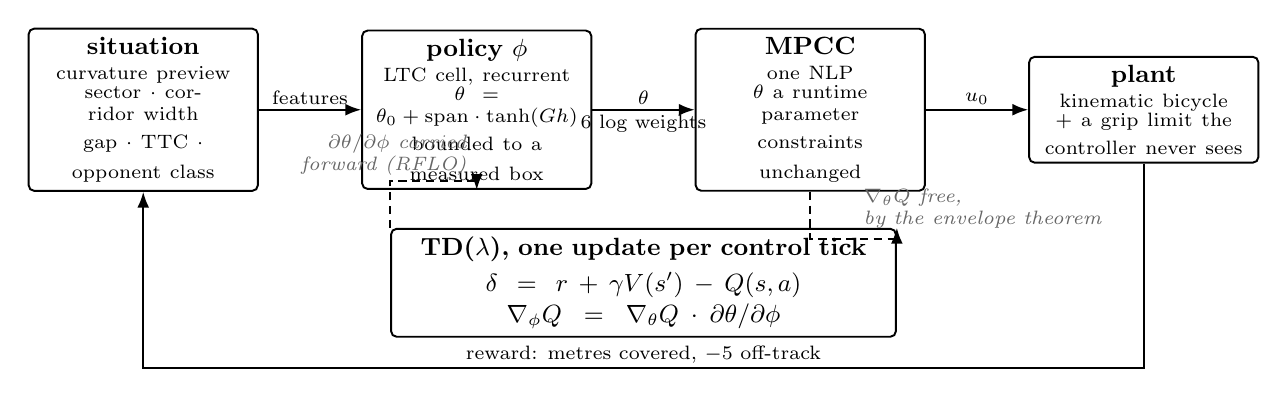
\begin{tikzpicture}[
      font=\small,
      box/.style   = {draw, rounded corners=2pt, line width=0.7pt,
                      minimum height=13mm, text width=27mm, align=center,
                      inner sep=3pt},
      sig/.style   = {-{Latex[length=2mm]}, line width=0.7pt},
      grad/.style  = {-{Latex[length=2mm]}, line width=0.7pt, densely dashed},
      lbl/.style   = {font=\scriptsize, inner sep=1.5pt},
      note/.style  = {font=\scriptsize\itshape, text=black!60},
    ]
    \node[box] (sit) {\textbf{situation}\\[1pt]
      \scriptsize curvature preview\\[-1pt]
      \scriptsize sector $\cdot$ corridor width\\[-1pt]
      \scriptsize gap $\cdot$ TTC $\cdot$ opponent class};
    \node[box, right=13mm of sit] (pol) {\textbf{policy} $\phi$\\[1pt]
      \scriptsize LTC cell, recurrent\\[-1pt]
      \scriptsize $\theta=\theta_0+\mathrm{span}\cdot\tanh(Gh)$\\[-1pt]
      \scriptsize bounded to a measured box};
    \node[box, right=13mm of pol] (mpc) {\textbf{MPCC}\\[1pt]
      \scriptsize one NLP\\[-1pt]
      \scriptsize $\theta$ a runtime parameter\\[-1pt]
      \scriptsize constraints unchanged};
    \node[box, right=13mm of mpc] (plant) {\textbf{plant}\\[1pt]
      \scriptsize kinematic bicycle\\[-1pt]
      \scriptsize $+$ a grip limit the\\[-1pt]
      \scriptsize controller never sees};

    \draw[sig] (sit) -- node[lbl, above]{features} (pol);
    \draw[sig] (pol) -- node[lbl, above]{$\theta$} node[lbl, below]{\scriptsize 6 log weights} (mpc);
    \draw[sig] (mpc) -- node[lbl, above]{$u_0$} (plant);

    \node[box, below=15mm of $(pol)!0.5!(mpc)$, text width=62mm] (td)
      {\textbf{TD($\lambda$), one update per control tick}\\[2pt]
       $\delta = r + \gamma V(s') - Q(s,a)$
       \qquad
       $\nabla_\phi Q = \nabla_\theta Q \cdot \partial\theta/\partial\phi$};

    \draw[grad] (mpc.south) -- ++(0,-6mm) -| (td.north east)
      node[note, pos=0.25, above right, align=left]
      {$\nabla_\theta Q$ free,\\by the envelope theorem};
    \draw[grad] (td.north west) -- ++(0,6mm) -| (pol.south)
      node[note, pos=0.75, above left, align=right]
      {$\partial\theta/\partial\phi$ carried\\forward (RFLO)};

    \coordinate (rb) at ($(plant.south)+(0,-26mm)$);
    \draw[sig] (plant.south) |- (rb) -| (sit.south)
      node[lbl, pos=0.25, above]{reward: metres covered, $-5$ off-track};
  \end{tikzpicture}
  \caption{The method. The controller stays an MPCC and its constraints are
  untouched; what is learned is a map from the situation to its six cost
  weights. The two dashed paths are the gradient: $\nabla_\theta Q$ falls out of
  the solve for free by the envelope theorem, and $\partial\theta/\partial\phi$
  must be carried forward because the policy is recurrent. That carry is the
  only approximation in the loop, and Section~\ref{sec:adapt} measures it as
  negligible (cosine $0.9997$ against exact RTRL).}
  \label{fig:arch}
\end{figure*}

Fig.~\ref{fig:arch} gives the whole loop; the subsections below give the parts.

\subsection{Situation-dependent weighting}
Let $\sigma : s \mapsto \{1,\dots,B\}$ label the track ahead. We hold one
$\theta_b$ per label and one tuner per label, and this second part is not
incidental: the eligibility trace belongs to the weights it accumulated for, so
a shared trace would credit a hairpin's gradient to the straight's weights. The
trace is reset at a label boundary and does not cross it.

The label is read from the path at a fixed preview distance ahead of the car
rather than at the car, so no detector and no estimator is involved --- the
schedule is \emph{observed}, and the comparison against a single $\theta$ is
therefore a comparison of parameterisations and not of perception.

\subsection{What the labels can and cannot be}\label{sec:sectors}
The obvious labelling is curvature, binned by quantiles of the track's own
$|\kappa|$ so the split transfers between geometries. \textbf{This cannot
express sector names.} For an arc of radius $R$, $\kappa = 1/R$ \emph{however
far the arc sweeps}, so a \SI{90}{\degree} corner and a \SI{180}{\degree}
hairpin of equal radius are identical to anything reading curvature at a point.
Measured on a circuit built with both at $R = \SI{2.6}{\meter}$: peak $|\kappa|$
agrees to within $2\%$ and the two fall in the same bin.

What separates them is the \emph{integral} of curvature through the corner. We
therefore detect a corner as an extended object --- a maximal run of $|\kappa|$
above a fraction of the track's peak --- and classify it by its total heading
change $\Delta\psi = \int \kappa\,\mathrm{d}s$ into straight, long curve
($|\Delta\psi| < \SI{60}{\degree}$), \SI{90}{\degree}
($\SI{60}{\degree} \le |\Delta\psi| < \SI{135}{\degree}$) and
\SI{180}{\degree}. The label belongs to the corner, not to the point, so it
cannot change part-way through a manoeuvre.

\begin{figure*}[t]
  \centering
  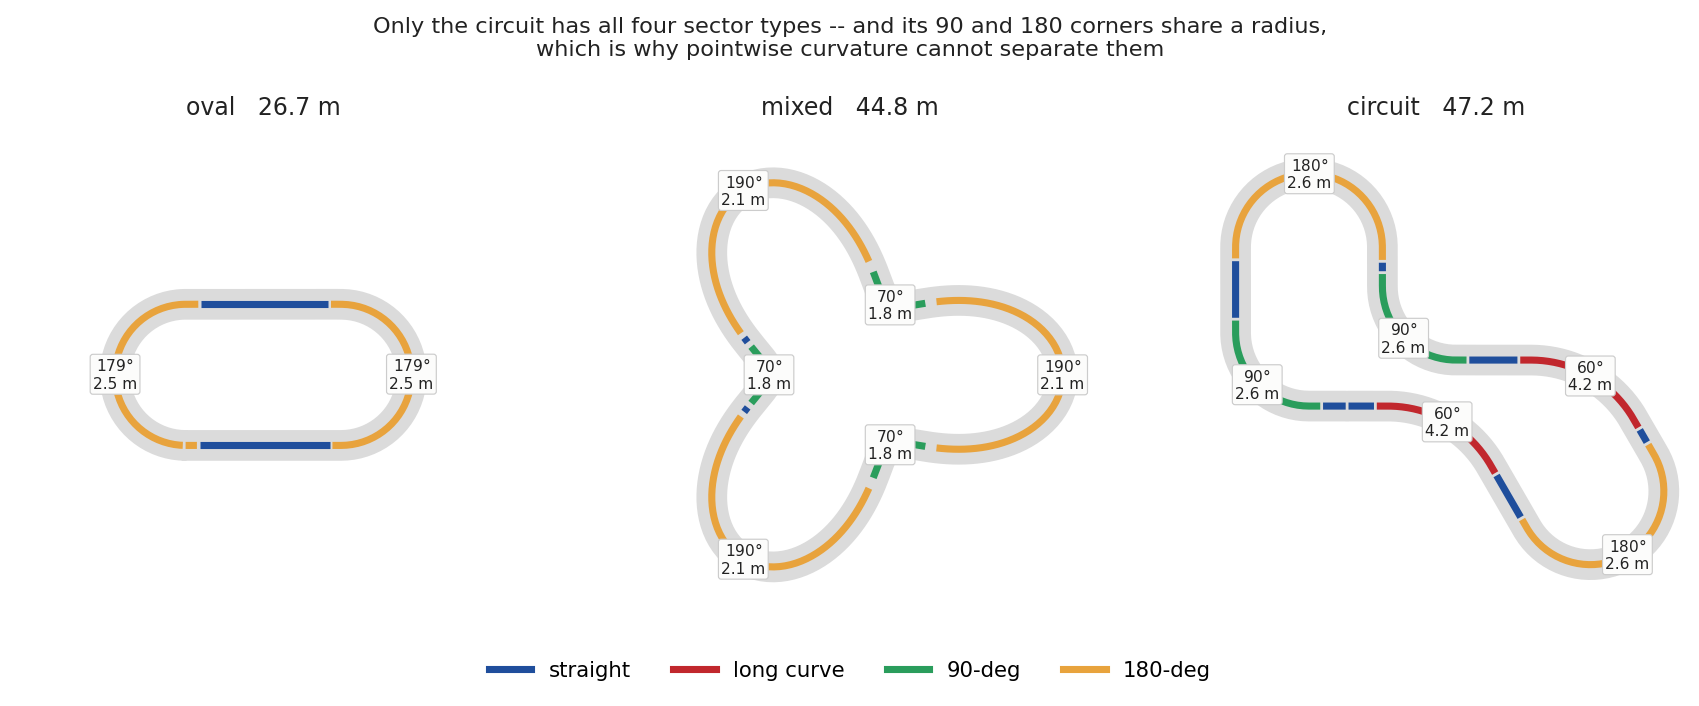
\includegraphics[width=\textwidth]{figures/tracks.png}
  \caption{The three tracks, coloured by named sector, drawn to a common scale.
  The oval has straights and two \SI{180}{\degree} corners; \texttt{mixed} adds
  \SI{90}{\degree} corners but no long curve; only \texttt{circuit} has all
  four. The circuit's \SI{90}{\degree} and \SI{180}{\degree} corners are built
  at the \emph{same radius} --- both labelled \SI{2.6}{\meter} --- which is
  exactly why curvature at a point cannot separate them.
  Reproduced by \texttt{scripts/make\_figures.py}.}
  \label{fig:tracks}
\end{figure*}

Fig.~\ref{fig:tracks} draws the three tracks under this labelling, and makes
the argument visible: the circuit's \SI{90}{\degree} and \SI{180}{\degree}
corners are built at the same radius, so nothing reading curvature at a point
can separate them.

We report the curvature-binned and sector-labelled schedules separately and do
not conflate them: \textbf{the six-seed result of Section~\ref{sec:seeds} is a
three-bin curvature schedule}, and calling it a sector schedule would overclaim.

\subsection{Obstacles, so that behaviour is expressible}
Without an obstacle in the OCP, ``overtake'' and ``follow'' are not two
behaviours the weights select between --- they are the same problem. We add
$M$ circular keep-outs as runtime parameters, softened with explicit slacks:
\begin{equation}
  \lVert p_k - o_j \rVert^2 - r_{\text{eff},j}^2 + s_{jk} \ge 0,
  \quad s_{jk}\ge 0,
  \label{eq:keepout}
\end{equation}
penalised $Z s^2 + z s$ in the cost, with $r_{\text{eff}} = r + m$ and inactive
slots passed as $r = -m$ so the constraint is exactly inert. Soft rather than
hard is deliberate: it makes ``stay behind'' a feasible finite-cost option, and
an infeasible solve is not a behaviour but a missing input.

The constraint is applied at nodes $1..N$ and not at node $0$, which is pinned
to the measurement --- a constraint there is a statement about the past, and it
would be unsatisfiable exactly when the car is already touching an opponent.

\subsubsection*{A car is not a circle}
A circular keep-out is wrong in both directions at once, and wrong in the one
that matters. A car is roughly $0.57 \times \SI{0.30}{\meter}$, so with the
standard margin at $r = \SI{0.20}{\meter}$ the semi-axes are
\SI{0.635}{\meter} along the opponent and \SI{0.267}{\meter} across it, against
a circle using \SI{0.350}{\meter} both ways: \SI{0.28}{\meter} too tight
\emph{alongside}, which is exactly where a pass happens, and \SI{0.29}{\meter}
too loose nose-to-tail. We therefore also implement the keep-out as an ellipse
aligned with the opponent's heading,
\begin{equation}
  (u/a)^2 + (v/b)^2 - 1 \;\ge\; 0,
  \label{eq:ellipse}
\end{equation}
with $u, v$ the displacement in the opponent's frame and the ego's own body
added to both semi-axes, so the constraint is between two rectangles rather
than between a point and one. Scaled by $ab$ so the row keeps the units of the
circular constraint and the slack weights remain comparable. Every
closest-approach figure reported here was measured against the circle, which is
the conservative choice for the numbers we quote.

\textbf{The slacks add decision variables and constraint rows, so we re-verify
the gradient rather than assume it survives}: with a keep-out active, the
envelope-theorem sensitivity agrees with central finite differences to cosine
$> 0.999$ and relative error $< 5\times10^{-2}$, the same thresholds as the
obstacle-free check.

\subsection{The behaviour policy}\label{sec:policy}
This subsection specifies the policy; Section~\ref{sec:gate} reports what
happened when it was run. The gate below was fixed \emph{before} the
experiment.

The target is a map $\phi : \text{situation} \to \theta$. Section~\ref{sec:axes}
constrains its shape in two ways that a design should respect rather than
rediscover: the behaviour boundary is a \emph{ratio} $q_v/q_c$, which because
$\theta$ is already a logarithm is a \emph{difference of two components of
$\theta$} and therefore a linear function of the output; and safety is set by
the magnitude of $q_v$, a different axis, so the output must be bounded by a
ceiling on $q_v$ rather than by a box.

\emph{Features}, eighteen of them, keyed on quantities with physical units so
that the map transfers between tracks and speeds: curvature preview at three
distances;
speed as a fraction of the cap; margin to the boundary; time-to-collision;
the lateral acceleration a pass would require against the grip left over after
cornering; and the gap to the car ahead, expressed \emph{both} against braking
distance $v^2/2a_{\max}$ and in absolute car lengths.

Three further groups carry the situation the weights are supposed to depend on.
The \textbf{named sector ahead} as a one-hot --- straight, long curve,
\SI{90}{\degree}, \SI{180}{\degree} --- read at a preview distance and
classified by the corner's total heading change, so the policy can hold a
different aggression for a hairpin than for a straight \emph{within one set of
parameters}, which is the continuous schedule Section~\ref{sec:sectors}
motivates. The \textbf{corridor width} in car widths, because whether a pass
fits is a property of the track and not only of the two cars. And the
\textbf{opponent class} as a one-hot: static, slower, equal, faster, graded by
\emph{relative} speed, because ``someone is \SI{2}{\meter} ahead'' means
opposite things depending on whether they are parked or pulling away.

That last group is the sharpest argument for a recurrent head. \textbf{Catching
and being caught are the same instantaneous gap with opposite signs of closing
rate, and they call for opposite behaviour}, so no function of a single frame
can separate them however many features it is given. The class is estimated
from observed positions by an exponential filter that requires three
observations before committing --- not read from the opponent's true speed,
which would delete the hidden state the recurrence exists for.

That the gap needs both is a correction we had to measure. A gap in braking
distances is the right quantity for ``can I stop'', but it is the wrong one for
``is this car close enough to engage'', because braking distance vanishes at low
speed: at \SI{1.4}{\meter\per\second} it makes a three-braking-distance
threshold \SI{0.54}{\meter}, while the keep-out itself holds the car
\SI{1.04}{\meter} away. \textbf{The engagement test then asks for a proximity
the safety constraint forbids}, and it fired on 0 of 400 ticks. Engagement is a
question about the geometry of two cars and is measured in car lengths.

\emph{The precondition that decides whether memory is needed.} If $\phi$ is
given the opponent's velocity, there is no hidden state and no temporal pattern,
and a recurrent head is decoration. A closing rate is a derivative of a range
and cannot be read from one frame, so \textbf{the temporal argument requires
deliberately withholding opponent velocity}, and we treat that as a design
choice to be defended rather than inherited.

\emph{Candidate heads.} Three, compared on identical features:
\begin{enumerate}
  \item a fixed schedule --- a lookup from sector and gap band;
  \item a per-tick MLP, memoryless;
  \item a liquid time-constant (LTC) cell~\cite{hasani2021ltc}, one step of
        \begin{equation}
          h^+ = \frac{h + \Delta t\, f(x,h)\,A}{1 + \Delta t\,(1/\tau + f(x,h))},
          \quad f = \sigma(W\xi),
          \label{eq:ltc}
        \end{equation}
        whose effective time constant $\tau_{\text{eff}} = \tau/(1 + \tau f)$ is
        set at run time by the input.
\end{enumerate}

The reason to consider \eqref{eq:ltc} specifically, rather than any recurrent
cell, is that $\tau_{\text{eff}}$ \emph{is} a hold duration: long when the gate
is shut, short when the input drives it. A behaviour decision should be taken
once and held --- re-deciding at \SI{20}{\hertz} invites chattering between
overtake and follow --- and a learned, situation-dependent hold is the
principled form of that, rather than a hand-set dwell time.

\emph{The gate, fixed in advance.} The recurrent head is claimed only if it
beats \emph{both} the fixed schedule and the per-tick MLP. We state a prediction
against ourselves: because the behaviour boundary is linear in $\theta$, the
fixed schedule should be strong, and the network can only win on the temporal
axis. Published results for this cell family on a closely related overtaking
task are \emph{not} favourable --- an LTC ranked sixth of seven cells and made
the fewest passes, below a memoryless MLP, though no cell in that comparison was
separated from another given the seed spread. We therefore regarded a negative
outcome as the likely one, and Section~\ref{sec:gate} is that outcome.

\subsection{Protocol}
The only stochastic element is actuator exploration noise, so a seed is a draw
of that stream and the plant, track and initialisation are deterministic; seed
variation measures the learner's reliability rather than the task's. Sweeps over
fixed weights are deterministic and single-run, and there each cell is exact
while the \emph{geometry} is $n=1$ --- we say which is which.

Episodes are 400 steps at \SI{20}{\hertz}. Three tracks: a \SI{26.7}{\meter}
oval (straights and two \SI{180}{\degree} corners); a \SI{47.2}{\meter}
synthetic circuit built to contain all four sector types, with a minimum radius
of \SI{2.59}{\meter} chosen to match the oval so a scheduling result is not
confounded by an initialisation failure; the Red Bull Ring at F1TENTH's
1:10 scaling (\SI{343}{\meter}, public \texttt{f1tenth\_racetracks} data); and
two circuits taken from the ICRA competition maps themselves --- the 2025 car10
track (\SI{204}{\meter} at the scale used here) and ICRA 2026 Track 1
(\SI{68.8}{\meter}, and the only track here carrying all four named sector
types). The last two are extracted directly from the teams' own ROS occupancy
grids; none of the three was designed by us. The third is not decoration: Section~\ref{sec:circuit}
is a demonstration that a conclusion reverses between the first two.

\section{When one weight vector is unstable}\label{sec:seeds}
Six seeds, 26 episodes each, on the oval. The only stochastic element is the
actuator exploration noise, so a seed is a draw of that stream and the spread
measures the learner's reliability rather than the task's.

\begin{table}[t]
  \centering
  \caption{One $\theta$ against one per curvature bin, six seeds, oval.
  ``Collapsed'' is a seed ending with at least half its final episodes
  off-track. \texttt{experiments/per\_segment\_seeds.py}.}
  \label{tab:seeds}
  \begin{tabular}{lrrr}
    \toprule
    & last 8 episodes & spread & collapsed \\
    \midrule
    one $\theta$          & \SI{8.9}{\meter}  & sd 0.9, 7.6--9.8   & \textbf{6 / 6} \\
    three curvature bins  & \textbf{\SI{77.8}{\meter}} & sd 0.2, 77.5--78.0 & \textbf{0 / 6} \\
    \bottomrule
  \end{tabular}
\end{table}

The distributions do not overlap: the \emph{worst} per-bin seed is eight times
the \emph{best} global one, and the per-bin spread of \SI{0.2}{\meter} is
tighter than the global one despite being nine times the magnitude.

\textbf{The mechanism is isolation, not expressive power}, and the best-episode
column is what shows it. A single $\theta$ reaches a \SI{77.6}{}--\SI{79.1}{\meter}
controller on \emph{every} seed and destroys it on \emph{every} seed, first
leaving the track at episode 3, 3, 4, 5, 5, 5. Per-bin weights reach the same
\SI{78.0}{}--\SI{78.3}{\meter} peak and keep it. The schedule does not find a
better policy; it removes the path by which a bad update in a corner reaches
the straight's weights.

\begin{figure*}[t]
  \centering
  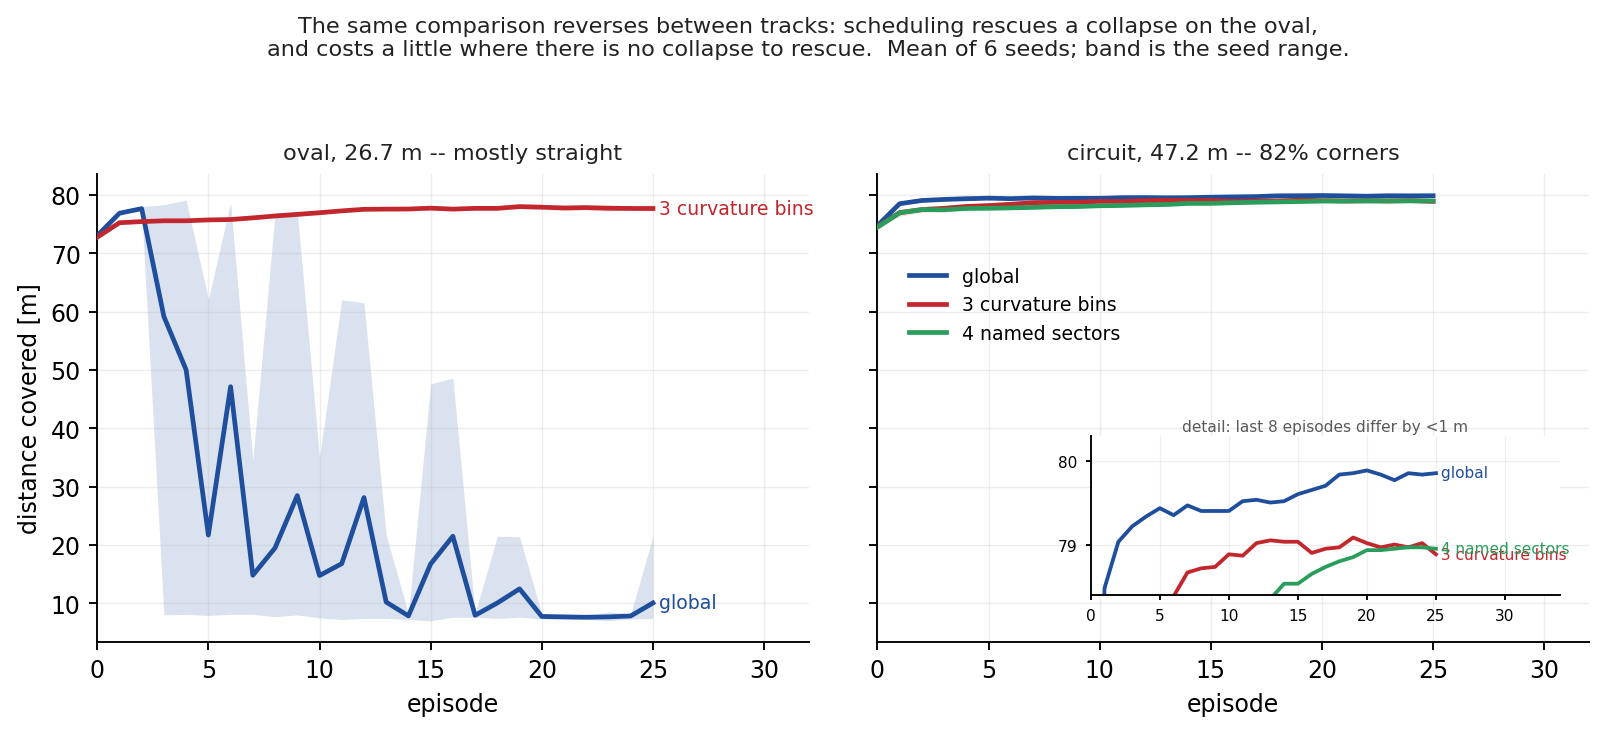
\includegraphics[width=\textwidth]{figures/reversal.png}
  \caption{The result reverses between tracks. \textbf{Left:} on the oval a
  single $\theta$ collapses on every seed while three curvature bins do not.
  \textbf{Right:} on the circuit nothing collapses, and the single $\theta$ is
  the \emph{best} of the three --- the inset resolves an ordering that spans
  less than \SI{1}{\meter} and would otherwise be invisible at the shared axis
  the comparison requires. Mean of six seeds; band is the seed range.
  Reproduced by \texttt{experiments/per\_segment\_seeds.py} and
  \texttt{experiments/per\_sector\_weights.py}.}
  \label{fig:reversal}
\end{figure*}

\subsection{And when it is not}\label{sec:circuit}
Fig.~\ref{fig:reversal} puts both tracks side by side; the panels are the same
measurement and land in different places. The same comparison on a
\SI{47.2}{\meter} circuit --- straights, a chicane of
two \SI{90}{\degree} corners, two \SI{180}{\degree} hairpins, a pair of
sweepers, minimum radius \SI{2.59}{\meter} --- reverses the result.

\begin{table}[t]
  \centering
  \caption{Six seeds on the circuit. The unscheduled controller wins, and the
  two scheduled variants are indistinguishable from each other.}
  \label{tab:circuit}
  \begin{tabular}{lrrrr}
    \toprule
    & $\theta$ & mean & sd & collapsed \\
    \midrule
    global          & 1 & \textbf{\SI{79.84}{\meter}} & 0.07 & 0/6 \\
    curvature bins  & 3 & \SI{78.99}{\meter}          & 0.19 & 0/6 \\
    named sectors   & 4 & \SI{78.92}{\meter}          & 0.07 & 0/6 \\
    \bottomrule
  \end{tabular}
\end{table}

Fig.~\ref{fig:overtake} shows that sweep with the boundary drawn.

Named sectors $-$ curvature bins is $\SI{-0.07}{\meter}$, $0.8$ SE: \textbf{not
separated}. Global $-$ curvature bins is $+\SI{0.85}{\meter}$ at $10.4$ SE and
global $-$ named sectors $+\SI{0.92}{\meter}$ at $22.5$ SE: both separated, and
in favour of \emph{fewer} parameters.

Two things follow. The collapse of Section~\ref{sec:seeds} is a property of the
\emph{track}: the oval is mostly straight, so the tuner is rewarded for raising
$q_v$ over most of the lap and then meets a \SI{180}{\degree} corner carrying
straight-tuned weights, whereas the circuit is $82\%$ non-straight and that
feedback arrives constantly. And with no collapse to prevent, extra weight
vectors are extra freedom for the tuner to wander with nothing to buy.

\textbf{The caveat is not small.} All three arms sit within \SI{1}{\meter} of
each other at the vehicle's \SI{4}{\meter\per\second} speed cap, with the
unmodelled grip limit active in the corners. This is a ceiling-limited task, so
``scheduling does not help here'' is measured and ``scheduling does not help''
is not. A task where scheduling has something to win --- conflicting demands
between sectors, or a speed range the cap does not truncate --- has not been
run.

\section{Behaviour is a ratio; safety is a magnitude}\label{sec:axes}
\begin{table}[t]
  \centering
  \caption{Outcome over the weight sweep, against an opponent \SI{3}{\meter}
  ahead at \SI{1}{\meter\per\second}. Runs are deterministic, so each cell is
  exact; the $n=1$ here is the \emph{geometry}, not the sampling.
  \texttt{experiments/overtake\_or\_follow.py}.}
  \label{tab:grid}
  \begin{tabular}{rrrrl}
    \toprule
    $q_v$ & $q_c$ & $q_v/q_c$ & covered & outcome \\
    \midrule
    0.5 & 10.0 & 0.05 & \SI{12.0}{\meter} & followed \\
    0.5 & 3.0  & 0.17 & \SI{12.0}{\meter} & followed \\
    0.5 & 1.0  & 0.50 & \SI{12.0}{\meter} & followed \\
    0.5 & 0.3  & 1.67 & \SI{22.3}{\meter} & passed \\
    0.5 & 0.1  & 5.00 & \SI{26.8}{\meter} & passed \\
    \midrule
    2.0 & 10.0 & 0.20 & \SI{12.0}{\meter} & followed \\
    2.0 & 3.0  & 0.67 & \SI{12.0}{\meter} & followed \\
    2.0 & 1.0  & 2.00 & \textbf{\SI{36.6}{\meter}} & passed \\
    2.0 & 0.3  & 6.67 & \textbf{\SI{36.8}{\meter}} & passed \\
    2.0 & 0.1  & 20.0 & \SI{3.3}{\meter}  & passed, then \textbf{off-track} \\
    \midrule
    10.0 & 10.0 & 1.00 & \SI{12.1}{\meter} & followed \\
    10.0 & 3.0  & 3.33 & \SI{2.3}{\meter} & passed, then \textbf{off-track} \\
    10.0 & 1.0  & 10.0 & \SI{3.1}{\meter} & passed, then \textbf{off-track} \\
    10.0 & 0.3  & 33.3 & \SI{3.7}{\meter} & passed, then \textbf{off-track} \\
    10.0 & 0.1  & 100  & \SI{3.5}{\meter} & passed, then \textbf{off-track} \\
    \bottomrule
  \end{tabular}
\end{table}

\textbf{The behaviour is the ratio.} Every cell with $q_v/q_c \le 1$ follows and
every cell above it passes --- fifteen of fifteen, across two decades in each
weight. Following is a settled behaviour rather than indecision: \SI{0.73}{\meter}
back, \SI{7}{\milli\meter} of lateral wander, held for the whole run. Since
$\theta$ is already the logarithm of the weights, this boundary is a
\emph{difference of two components of $\theta$}, and therefore linear in the
policy's output --- which is why we predict a linear schedule to be a strong
baseline in Section~\ref{sec:gate}.

\textbf{Safety is $q_v$ alone, and it is a different axis.} The ratio does not
predict survival: $q_v/q_c = 5.0$ completes the lap and $3.33$ leaves the track.
Sorted by $q_v$ it is immediate --- every pass at $q_v = 10$ goes off, one of
two at $q_v = 2$, none at $q_v = 0.5$. So the region a learned policy must be
confined to is \textbf{not a box in $\theta$ and not a bound on the ratio}: it
is a ceiling on $q_v$ with the ratio left free.

\textbf{The keep-out never failed.} No run ended in a collision and the minimum
clearance across every step was $+\SI{0.123}{\meter}$ outside $r$. All five
failures are track-limit failures --- running wide \emph{while} passing --- which
is a distinction available only because the plant records which failure
occurred.

\begin{figure}[t]
  \centering
  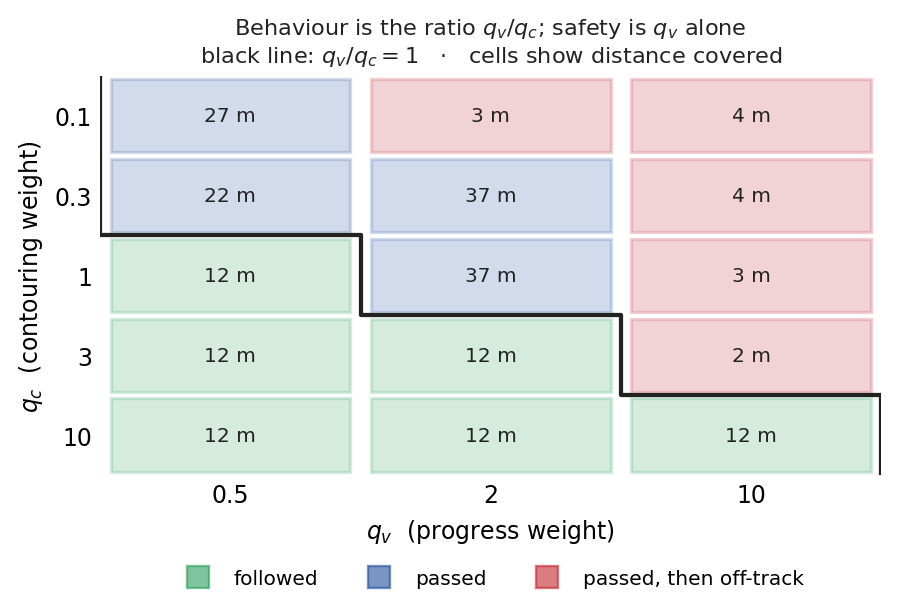
\includegraphics[width=\columnwidth]{figures/overtake_grid.png}
  \caption{Outcome over the weight sweep, against an opponent \SI{3}{\meter}
  ahead at \SI{1}{\meter\per\second}. Every cell below the line follows and
  every cell above it passes, so the behaviour boundary is the ratio
  $q_v/q_c$. Whether the pass \emph{survives} is set by $q_v$ alone: the whole
  $q_v = 10$ column leaves the track. The outcome is categorical, so the cells
  are a labelled state grid and not a heat map --- a sequential ramp would
  imply an ordering between ``followed'' and ``crashed'' that does not exist.
  Reproduced by \texttt{experiments/overtake\_or\_follow.py}.}
  \label{fig:overtake}
\end{figure}

\section{The behaviours, on a circuit we did not design}\label{sec:behaviour}

Every track above is synthetic and built here, and Section~\ref{sec:circuit} is
itself a demonstration that a conclusion can reverse between two such tracks. We
therefore repeat the behaviour measurement on the Red Bull Ring at
F1TENTH's 1:10 scaling, from the public \texttt{f1tenth\_racetracks} data.

The choice is not only about provenance. On our synthetic circuit the tightest
corner admits \SI{3.9}{\meter\per\second} against the vehicle's
\SI{4}{\meter\per\second} cap, so the car sits flat out for the whole lap and
every weight setting lands within \SI{1}{\meter} of every other: the task cannot
discriminate. Spielberg's tightest corner admits
\SI{2.5}{\meter\per\second}, so the controller must modulate speed and the
weights have something to do --- three settings gave $45.9$, $54.3$ and
\SI{57.6}{\meter}.

\begin{figure}[t]
  \centering
  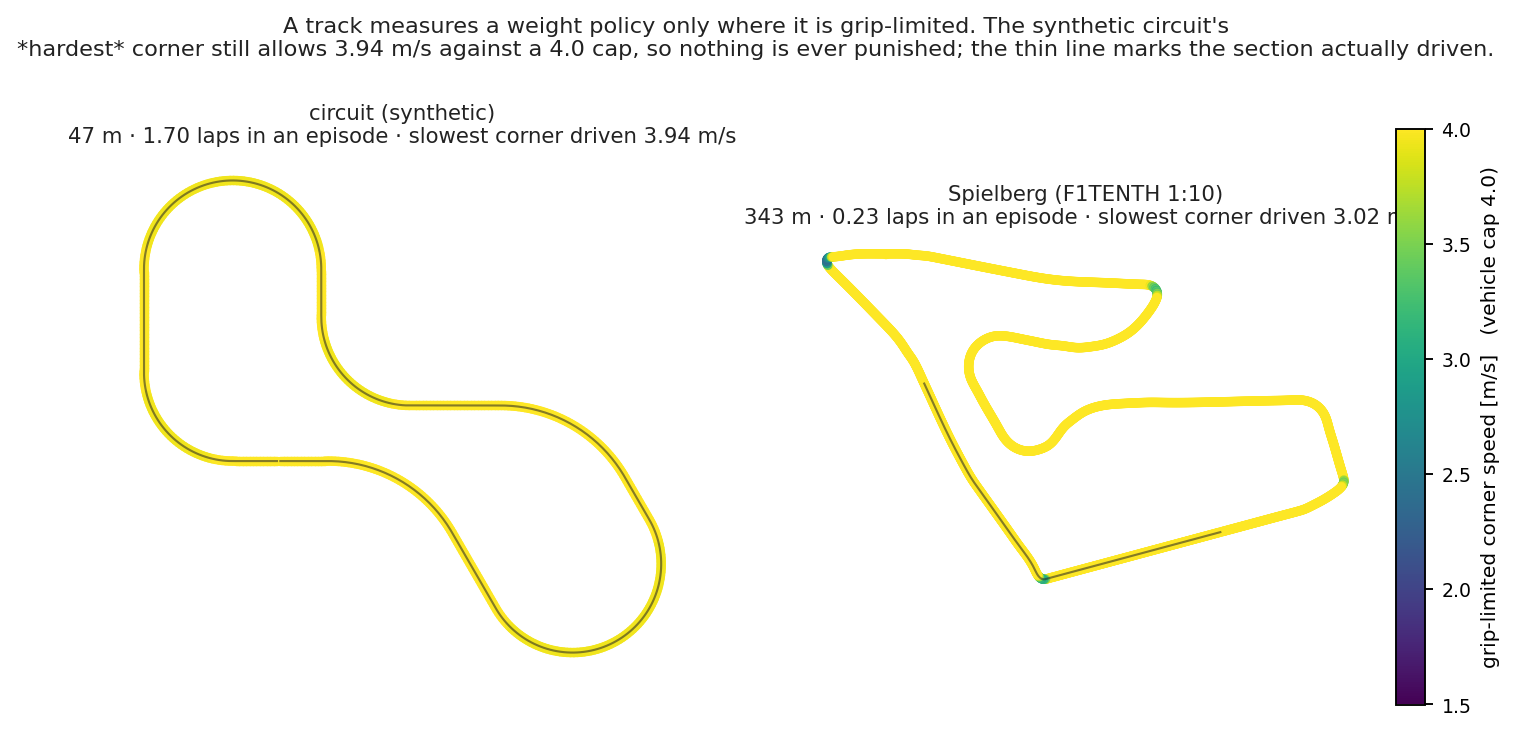
\includegraphics[width=\columnwidth]{figures/spielberg.png}
  \caption{A track measures a weight policy only where it is grip-limited.
  Colour is $\sqrt{a_{\text{lat,max}}\mu/\kappa}$ against the vehicle's
  \SI{4}{\meter\per\second} cap; the thin line is the section driven in one
  episode. The synthetic circuit's \emph{hardest} corner still allows
  \SI{3.94}{\meter\per\second}, so no weight setting is ever punished. Note the
  naive metric points the wrong way --- Spielberg is at the cap for $97\%$ of
  its lap and the circuit for $58\%$ --- because what matters is the minimum
  reached, not the fraction.}
  \label{fig:spielberg}
\end{figure}

Two weights carry behaviour. Following is a ratio $q_v/q_c$ below one and
overtaking a ratio above it; \emph{aggression} scales how hard the behaviour is
pursued without crossing that boundary. Crossing it is a change of behaviour,
not of intensity. Three postures are compared: never pass, pass only when the
manoeuvre is physically available, and always attempt it.

\begin{table}[t]
  \centering
  \caption{Three postures by three aggressions, Spielberg, one slower opponent,
  three seeds, against a moving car and a stopped one. Zero collisions in 54
  runs and closest approach $+\SI{0.056}{\meter}$ outside the keep-out --- but
  see Section~\ref{sec:static}: the \SI{5.6}{\meter} rows are a livelock, so
  zero crashes conceals a failure here rather than demonstrating safety.}
  \label{tab:behaviour}
  \begin{tabular}{llrrr}
    \toprule
    posture & aggression & covered & passes & switches \\
    \midrule
    stay behind        & cautious   & \SI{33.6}{\meter} & 0.00 & 0.0 \\
    stay behind        & neutral    & \SI{34.7}{\meter} & 0.00 & 0.0 \\
    stay behind        & aggressive & \SI{34.7}{\meter} & 0.00 & 0.0 \\
    overtake when safe & cautious   & \SI{33.6}{\meter} & 0.00 & 1.3 \\
    overtake when safe & neutral    & \SI{54.7}{\meter} & 0.67 & 2.0 \\
    overtake when safe & aggressive & \textbf{\SI{74.6}{\meter}} & \textbf{1.00} & 2.0 \\
    always try         & cautious   & \SI{33.6}{\meter} & 0.00 & 0.7 \\
    always try         & neutral    & \SI{54.7}{\meter} & 0.67 & 1.7 \\
    always try         & aggressive & \SI{74.6}{\meter} & 1.00 & 2.0 \\
    \midrule
    \multicolumn{5}{l}{\emph{against a \textbf{static} obstacle}} \\
    stay behind        & cautious / neutral & \SI{5.6}{\meter} & 0.00 & 1.0 \\
    overtake when safe & cautious / neutral & \SI{5.6}{\meter} & 0.00 & 2.0 \\
    always try         & cautious / neutral & \SI{5.6}{\meter} & 0.00 & 1.0 \\
    stay behind        & aggressive & \SI{75.0}{\meter} & 1.00 & 2.0 \\
    overtake when safe & aggressive & \SI{75.2}{\meter} & 1.00 & 2.0 \\
    always try         & aggressive & \SI{75.0}{\meter} & 1.00 & 2.0 \\
    \bottomrule
  \end{tabular}
\end{table}

\textbf{The behaviours are expressible and the effect is large.} Following
covers \SI{34}{\meter}; overtaking at high aggression covers
\SI{74.6}{\meter} --- $2.2\times$ --- with one pass per episode and no crashes,
from moving two cost weights while the MPCC enforces every constraint
unchanged.

\textbf{But aggression is the axis that matters, and the posture is not.} The
two overtaking postures differ in what they \emph{decide} --- the switch counts
separate, so the availability gate does fire --- and are identical in what they
\emph{achieve}, to three significant figures. We attribute this to the
experiment rather than to the policy: one slower car on a wide circuit makes a
pass almost always available, so ``when safe'' and ``always'' should coincide.
Separating them needs a case where the pass is genuinely unavailable, and we do
not have one. The claim that a weight policy can express \emph{safe} overtaking
is therefore \textbf{not} established here; only that it can express overtaking.

\begin{figure}[t]
  \centering
  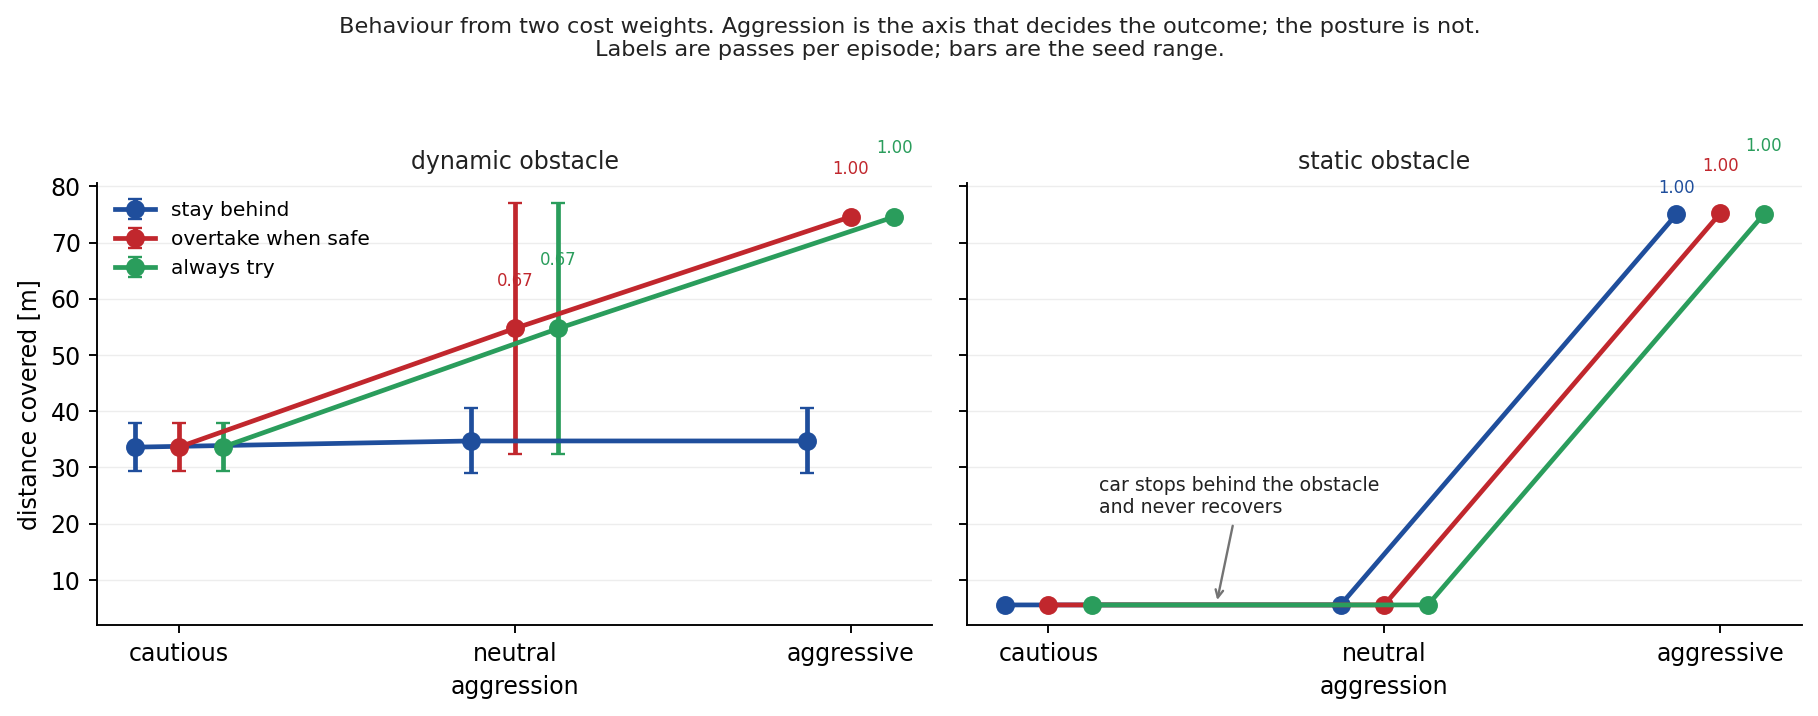
\includegraphics[width=\columnwidth]{figures/behaviour.png}
  \caption{Behaviour from two cost weights, against a moving car and against a
  stopped one. Aggression decides the outcome; the posture does not. The floor
  at \SI{5.6}{\meter} in the right panel is a livelock, not a slow lap: the car
  parks behind the static obstacle and the episode times out.
  \texttt{experiments/behaviour\_modes.py}.}
  \label{fig:behaviour}
\end{figure}

\begin{figure}[t]
  \centering
  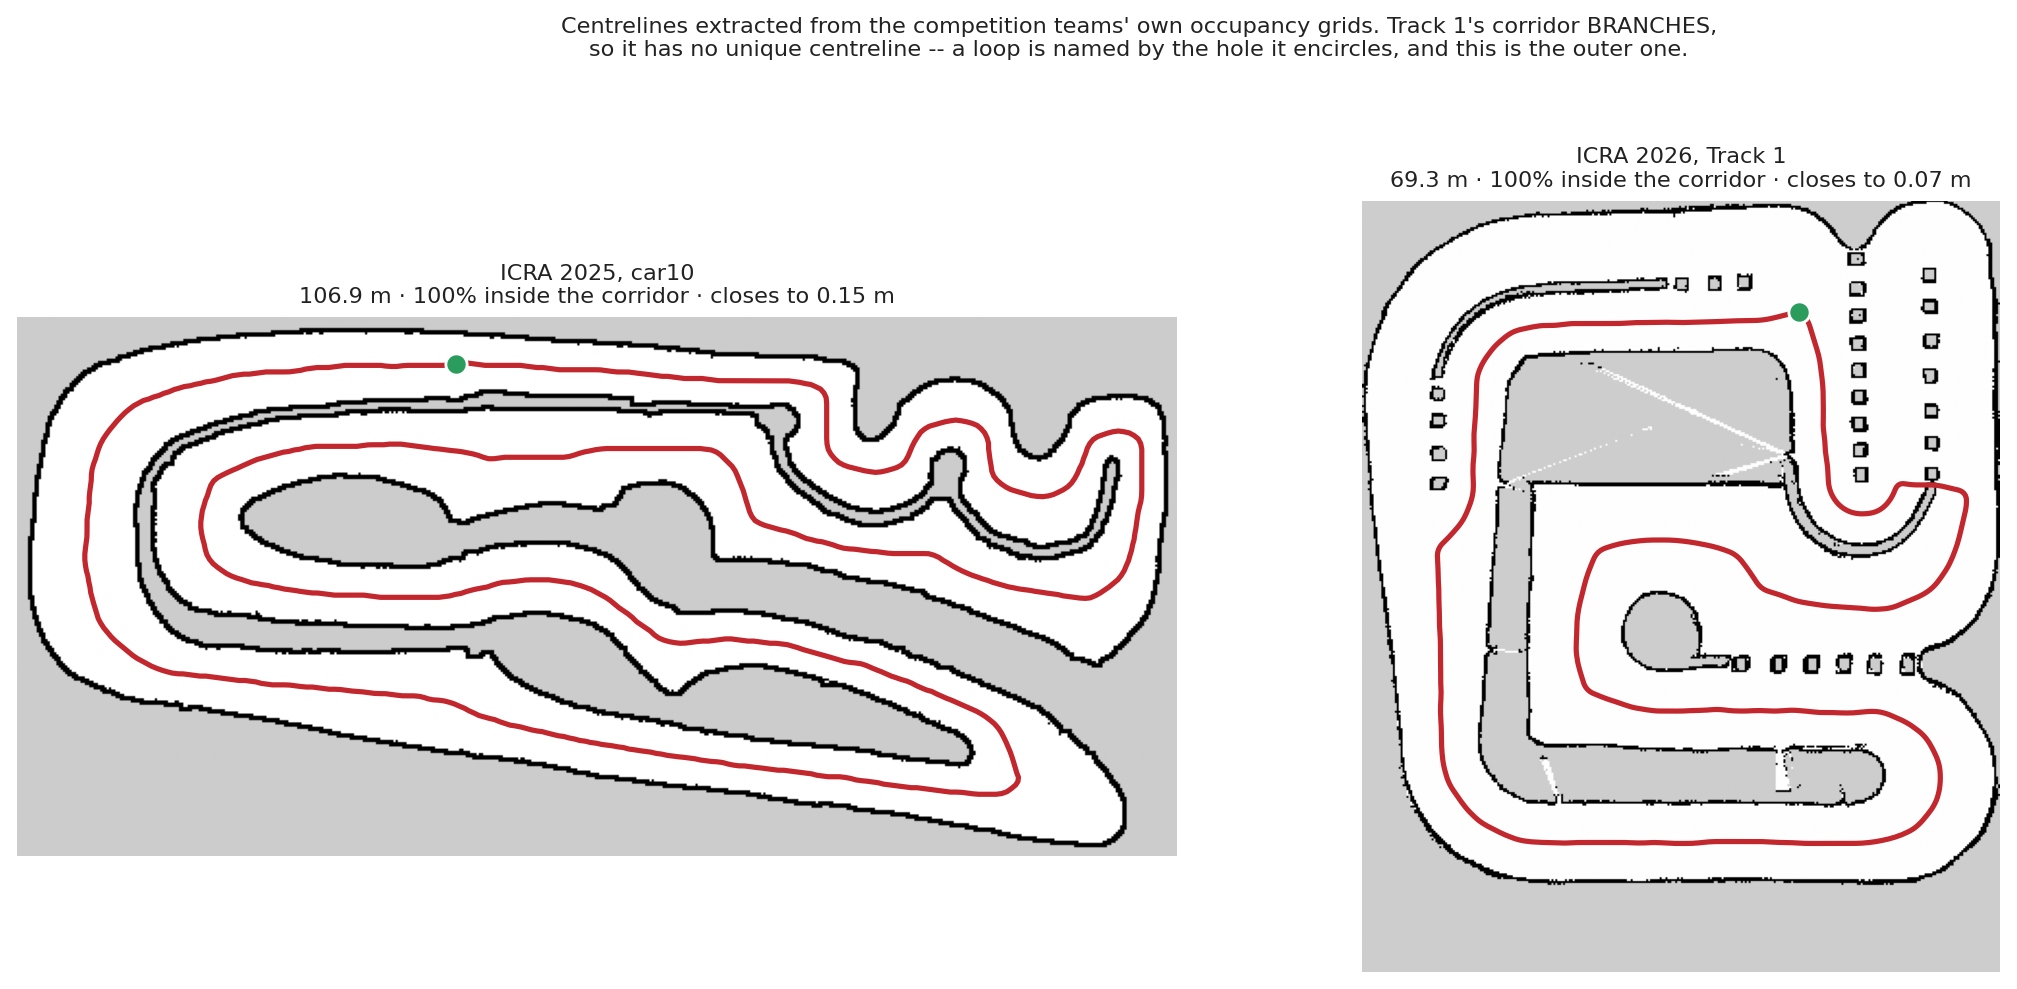
\includegraphics[width=\columnwidth]{figures/icra_tracks.png}
  \caption{Centrelines extracted from the competition teams' own ROS occupancy
  grids, at 100\% inside the corridor. Track 1's corridor \emph{branches} --- an
  outer ring plus an inner section --- so it has no unique centreline; a loop is
  named by the hole it encircles, and this is the outer one. Track 1 is also
  the only circuit here carrying all four named sector types. Rows of cones are
  \emph{welded} into continuous wall before extraction (orange): a cone row is
  a boundary whose area is mostly the free space between the cones, so the
  hole-filling the skeleton requires had been turning a wall into driveable
  track, and the extracted line was free to cross it. After welding, no point
  of the centreline lies inside a weld and the nearest clears it by
  \SI{0.70}{\meter} against a \SI{0.12}{\meter} car half-width.
  \texttt{tools/centerline\_from\_map.py}.}
  \label{fig:icra}
\end{figure}

Two of the tracks are taken directly from the ICRA competition maps
(Fig.~\ref{fig:icra}) rather than designed here, which matters because
Section~\ref{sec:circuit} is itself a demonstration that a conclusion can
reverse between two tracks that were.

\subsection{A stopped car is not a slow car}\label{sec:static}
``Stay behind'' is a behaviour only against something that is going somewhere.
Behind a \emph{static} obstacle it is not caution, it is stopping. The posture
must therefore be conditioned on a classification, and \textbf{that
classification cannot be made from a single frame} --- a stopped car and a slow
car are identical in one observation, and only their positions over time
differ. We estimate it from observed positions with an exponential filter that
requires three observations before it will commit; it is not given the
opponent's true speed. It classified correctly on $100\%$ of moving runs and
$0\%$ of stationary ones.

This is a stronger argument for a recurrent policy than a closing rate, because
it \emph{gates the entire behaviour choice} rather than tuning it, and it is
what a detection-and-tracking stack supplies on a vehicle.

Table~\ref{tab:behaviour} and Fig.~\ref{fig:behaviour} give the result, and it
is not the one we expected. With the classification in place ``stay behind''
correctly goes around a stopped obstacle (\SI{75.0}{\meter}, one pass). But
\textbf{at cautious and neutral aggression every posture stalls at
\SI{5.6}{\meter}}: the car parks behind the obstacle and the episode times out.
Two of three settings livelock, and no run in the entire study crashed --- so a
crash rate of zero here conceals a failure rather than demonstrating safety.

The mechanism is a trap worth naming. Our availability test requires a closing
speed. As the car slows toward a static obstacle the closing speed tends to
zero, so the test reports no pass available, so the car keeps following, so it
stops --- \textbf{and once stopped it can never authorise the manoeuvre that
would restore the motion the test demands}. Escaping it required
$q_c \le 0.5$: a static obstacle sits \emph{on} the reference line
permanently, so the contouring weight must yield before the car will leave the
line at all, and that threshold is lower than the one that suffices to pass a
moving car.

\begin{figure}[t]
  \centering
  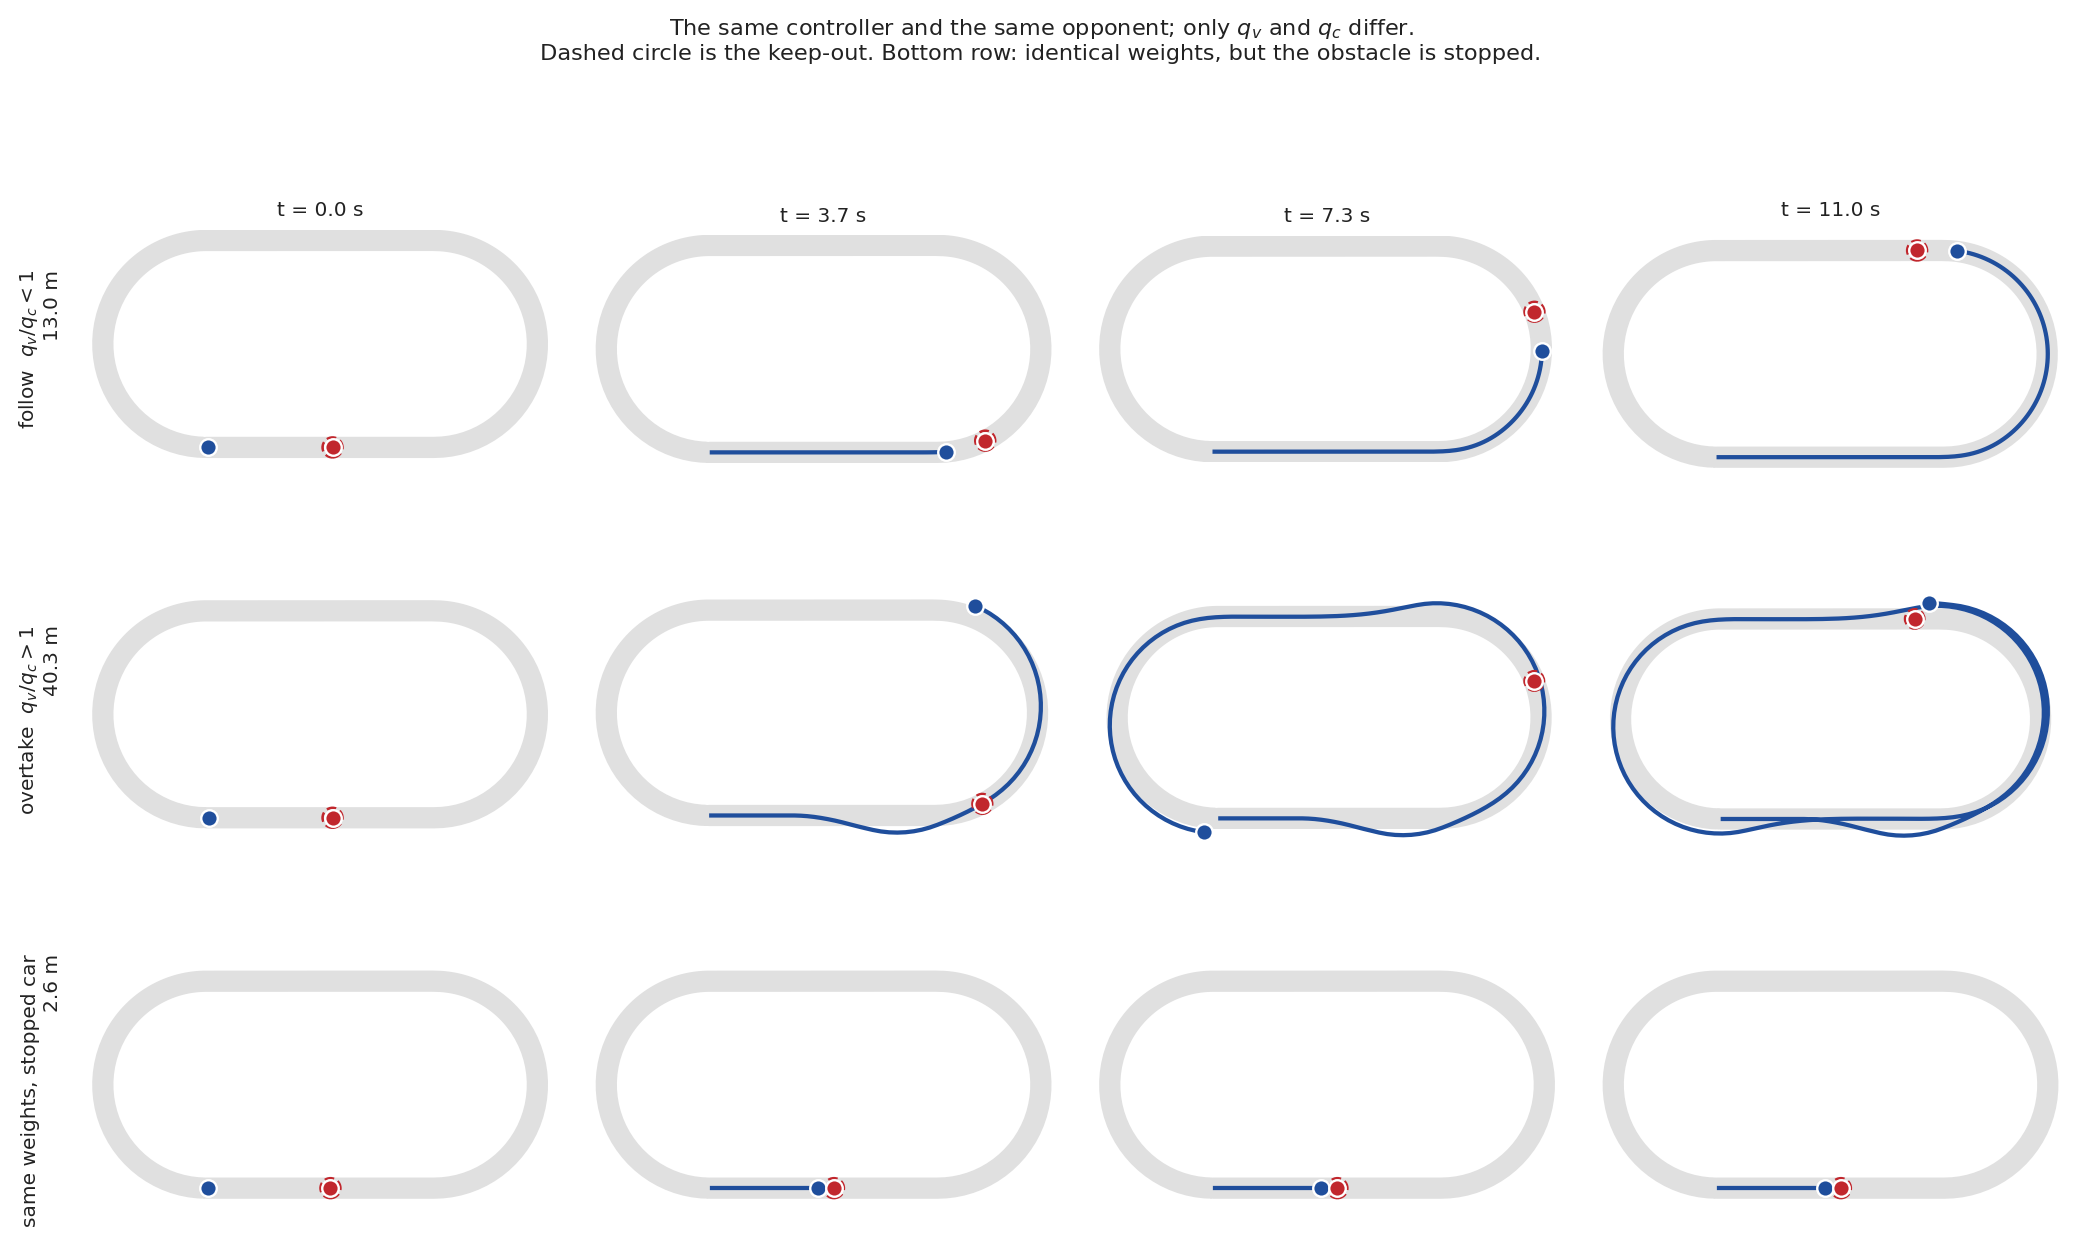
\includegraphics[width=\columnwidth]{figures/filmstrip.png}
  \caption{The same three runs as stills, since a PDF cannot hold an animation.
  Rows: following, overtaking, and the \emph{same} following weights against a
  stopped obstacle. Dashed circle is the keep-out. The bottom row is the
  livelock --- the car parks and the episode times out.}
  \label{fig:film}
\end{figure}

Fig.~\ref{fig:film} shows the three cases as trajectories over time.

\subsection{Three defects, and what found them}
Each was silent, and each produced a table that looked like a result.

\emph{Aggression crossed the behaviour boundary.} Scaling $q_c$ and $q_v$
oppositely put ``cautious overtake'' at a ratio of $0.71$, below one, so it
followed --- measured, byte-identical to never passing.

\emph{The ceiling and the dial collided.} With $q_v$ clipped at the measured
safe ceiling, aggressive and neutral overtaking became the same weights. Above
neutral, aggression now acts on $q_c$: caring less about the racing line rather
than wanting more speed, which is what the ceiling leaves available.

\emph{The engagement test was denominated in braking distance}, which vanishes
at low speed. At \SI{1.4}{\meter\per\second} it demanded a \SI{0.54}{\meter}
gap while the keep-out holds the car at \SI{1.04}{\meter} --- \textbf{it asked
for a proximity the safety constraint forbids}, and fired on 0 of 400 ticks.
Engagement is a question about the geometry of two cars and is now measured in
car lengths.

Only the third mattered. We report all three because the first two were
\emph{fixed first}, the table did not move, and a re-run is what revealed that
the diagnosis was wrong --- and because a safety-relevant component that is
silently inert reads as working rather than as broken, which is the same failure
mode this project has recorded before in its safety filters.

\section{Does the recurrence earn its place?}\label{sec:gate}

Section~\ref{sec:policy}'s gate, run. Four arms on the oval with one slower
opponent, identical in everything except what emits $\theta$: one global
$\theta$ tuned by TD($\lambda$); the hand-written schedule; a memoryless MLP;
and the LTC. Both networks are trained by the \emph{same} rule --- the
envelope gradient $\mathrm{d}Q/\mathrm{d}\theta$ chained through the policy to
$\mathrm{d}Q/\mathrm{d}\phi$, with the influence of the recurrent state carried
in RFLO form $P \leftarrow \text{leak}\cdot P + \text{imm}$. For the LTC that
leak is $1/(1+\Delta t(1/\tau + f)) < 1$ \emph{structurally}, guaranteed by
$1/\tau > 0$: the cell cannot learn to hold its state perfectly and so cannot
make the influence series diverge, which elsewhere requires an arbitrary cap.

\begin{table}[t]
  \centering
  \caption{The gate. Five seeds, twenty runs. Distance and crashes must be read
  together: an arm that passes more by crashing more has not done better.}
  \label{tab:gate}
  \begin{tabular}{lrrrr}
    \toprule
    & covered & sd & passes & crashes \\
    \midrule
    one $\theta$          & \SI{18.8}{\meter} & 4.6 & 0.33 & $22\%$ \\
    \textbf{fixed schedule} & \textbf{\SI{36.3}{\meter}} & \textbf{2.1} & 1.02 & $\mathbf{35\%}$ \\
    per-tick MLP          & \SI{27.2}{\meter} & 6.8 & \textbf{1.43} & $80\%$ \\
    LTC (recurrent)       & \SI{24.0}{\meter} & 13.7 & 1.35 & $78\%$ \\
    \bottomrule
  \end{tabular}
\end{table}

\begin{figure}[t]
  \centering
  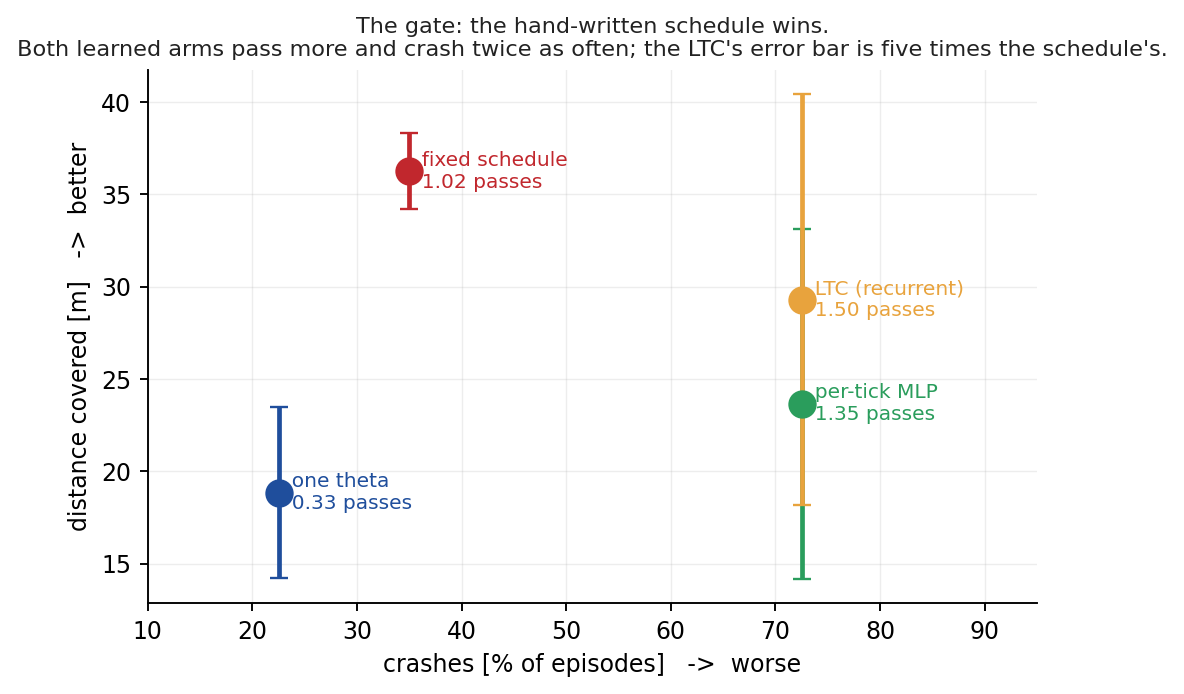
\includegraphics[width=\columnwidth]{figures/ltc_gate.png}
  \caption{The gate, as the two measures that must be read together. The
  hand-written schedule is up and to the left. Both learned arms pass more and
  crash twice as often, and the LTC's error bar is five times the schedule's.}
  \label{fig:gate}
\end{figure}

Fig.~\ref{fig:gate} plots the two measures against each other, which is how
they have to be read: an arm that passes more by crashing more has not done
better.

\textbf{Verdict: not claimed} --- and Section~\ref{sec:degenerate} shows the
comparison is weaker still than that, because both learned arms collapse to
constants. $\text{LTC} - \text{fixed} = -\SI{12.3}{\meter}$
at $2.0$ SE and $\text{LTC} - \text{MLP} = -\SI{3.3}{\meter}$ at $0.5$ SE. The
first gap \emph{is} separated, so on this task the recurrent policy is not
merely unproven against a fifteen-line lookup --- it is measurably worse than
one.

Three things are worth more than the verdict.

\emph{The hand-written schedule wins, and it is not a straw man}: it encodes
the $q_v/q_c$ boundary measured in Section~\ref{sec:axes}. A baseline with the
measurement built into it is a far harder target than a heuristic, and that is
much of why learning loses here.

\emph{The variance is the tell.} Its standard deviation is six times the
schedule's. That is the failure reported for this cell family elsewhere --- not
uniformly worse, but less reliable --- and Section~\ref{sec:adapt} shows what
produces it here.

\emph{Learning made the controller more reckless, which inverts the companion
result.} On a closely related task every learned cell roughly halved a scripted
policy's crash rate; here the scripted policy crashes $35\%$ of episodes and
both learned arms $72\%$. The action space plausibly explains it: there the
network emits steering and can learn to avoid, whereas here it emits cost
weights and the way to overtake is to raise $q_v$, which is also the way to
leave the track.

\section{What the policy actually does online}\label{sec:adapt}

A table of four arms says which won. It cannot show the thing the method is
about --- that $\theta$ is a function of the situation, re-emitted every tick.
Fig.~\ref{fig:adapt} draws what the policy emitted while it learned, and it is
the most informative result in this paper because it is the one that found the
bugs.

\begin{figure}[t]
  \centering
  
\includegraphics[width=\columnwidth]{figures/adaptation.png}
  \caption{The LTC policy over twelve episodes of online learning against one
  opponent. \textbf{Left:} the driven path coloured by the ratio $q_v/q_c$ the
  policy chose at each tick, diverging about the measured behaviour boundary of
  $1.0$. \textbf{Right, top:} the two weights through one lap, with the
  measured $q_v$ ceiling. \textbf{Right, bottom:} distance per episode. The
  policy drives $q_v$ onto its ceiling and $q_c$ towards zero; the ratio
  saturates near $22$, twenty times past the boundary, and the return collapses
  with it. \texttt{scripts/make\_figures.py}.}
  \label{fig:adapt}
\end{figure}

\subsection{The policy degenerates to a constant}\label{sec:degenerate}
Drawing the emitted weights was not enough on its own, because a flat trace can
be read as ``it settled''. The decisive measurement is a sensitivity sweep:
train the policy, freeze it, then vary one feature group at a time and record
the $\theta$ it emits.

\begin{table}[t]
  \centering
  \caption{Spread of the emitted $q_v/q_c$ when one feature group is swept and
  the rest held neutral, after training. Three seeds.
  \texttt{experiments/feature\_sensitivity.py}.}
  \label{tab:sens}
  \begin{tabular}{lrr}
    \toprule
    feature group & spread & relative \\
    \midrule
    named sector      & 0.46 & $1.9\%$ \\
    opponent class    & 0.34 & $1.4\%$ \\
    curvature preview & 0.21 & $0.9\%$ \\
    gap               & 0.40 & $1.7\%$ \\
    corridor width    & 0.05 & $0.2\%$ \\
    \bottomrule
  \end{tabular}
\end{table}

The trained policy emits $q_v/q_c \approx 19.8$ \emph{whatever it is shown}.
Across all four sectors: $19.83, 19.94, 19.36, 20.22$. Across all four opponent
classes: $20.30, 19.83, 19.93, 19.73$. \textbf{It is not a policy; it is a
constant, and all eighteen features are decorative.} Every comparison in
Section~\ref{sec:gate} is therefore between two constants, and should be read
as such.

\textbf{The output parameterisation is not the cause --- retracted; see
Section~\ref{sec:deadspan}.} We tried three --- a hard clip, a $\tanh$ centred
on the feasible box, and a $\tanh$ anchored at the reference controller with
asymmetric span --- and all three end at $q_v/q_c \approx 19.7$ with the
features ignored. The untrained policy is
responsive (ratio $0.70$--$0.95$ over random inputs); \emph{training} is what
destroys it. TD($\lambda$) drives $\theta$ monotonically, $\theta$ reaches
whichever bound exists, the squash saturates there, the output stops responding
to its input, and the policy collapses. Each bound changed \emph{where} it
saturates and never \emph{whether}.

This is the failure our companion work documents for a \emph{single} global
$\theta$~\cite{paper1} --- a proxy optimised past the point where the proxy is
valid, with nothing to stop it --- inherited whole by a policy over $\theta$. No
bound on the output can repair it, because the deficiency is that nothing makes
stopping preferable to continuing. \textbf{A stopping criterion is a
prerequisite for this line of work, not an improvement to it}, and we would not
run another policy comparison without one.

\subsection{A structural cause, and what it makes
provisional}\label{sec:deadspan}
The paragraph above is wrong, and the way it is wrong is worth reporting.

The third parameterisation anchors the output at the reference controller
$\theta_0$ and gives it an asymmetric span,
%
\begin{equation}
  \theta = \theta_0 + s(t)\,t, \qquad
  s(t) = \begin{cases} \theta_{\max} - \theta_0, & t \ge 0\\
                       \theta_0 - \theta_{\min}, & t < 0\end{cases}
  \label{eq:span}
\end{equation}
%
with $t = \tanh(Gh)$, so the policy gradient carries a factor
$\partial\theta/\partial z = (1 - t^2)\,s(t)$. We had set $\theta_0$ to the
offline-tuned weights \emph{deliberately} --- the offline parameters are meant
to be stable and the online policy adjusts around them --- and had drawn the
box from measurements of where each weight stops helping. Two of those
coincided: $q_l$ at $200$ and $q_v$ at $2.0$ were each equal to their own
ceiling, so $s(t) = 0$ for $t \ge 0$ and the gradient through both weights was
\emph{identically zero} whenever the pre-activation was non-negative. Half the
time, structurally, the two weights had no learning signal and could only be
revised downward.

$q_v$ is the weight that carries behaviour, through the ratio $q_v/q_c$, and
safety, through its magnitude. The most consequential parameter in the policy
was the half-dead one. This also accounts for the signature every
hypothesis we tested shared and none explained --- the output pinned at
\emph{a bound}, at $0.006$, $0.100$, $19.8$ and $39.97$ across configurations
--- and for Fig.~\ref{fig:driving}, where $q_v$ sits flat on the ceiling it
could not be pushed off.

We therefore mark as \textbf{provisional} every result in this section, the
gate comparisons of Section~\ref{sec:gate}, and our adaptation of RTRRL's
entropy regulariser~\cite{lemmel2023rtrrl} (which moved the output off its
bound, $0.006 \to 1.733$, but bought no situation-dependence and halved
distance covered, $4.9 \to 2.3$). All were measured on a policy whose behaviour
weight could move one way only. The box has been widened so every anchor is
strictly interior, and the policy now refuses to construct with an anchor on a
bound; the re-measurement is not in this version.

We are explicit that this does \emph{not} retract the stopping-criterion
argument, which stands on its own evidence, and does not yet establish that the
dead span was the sole cause. It establishes that a mechanism sufficient to
produce the observed collapse was present throughout, and that the earlier
elimination of the output map was performed on an instance of the output map
that was itself broken.

\begin{figure*}[t]
  \centering
  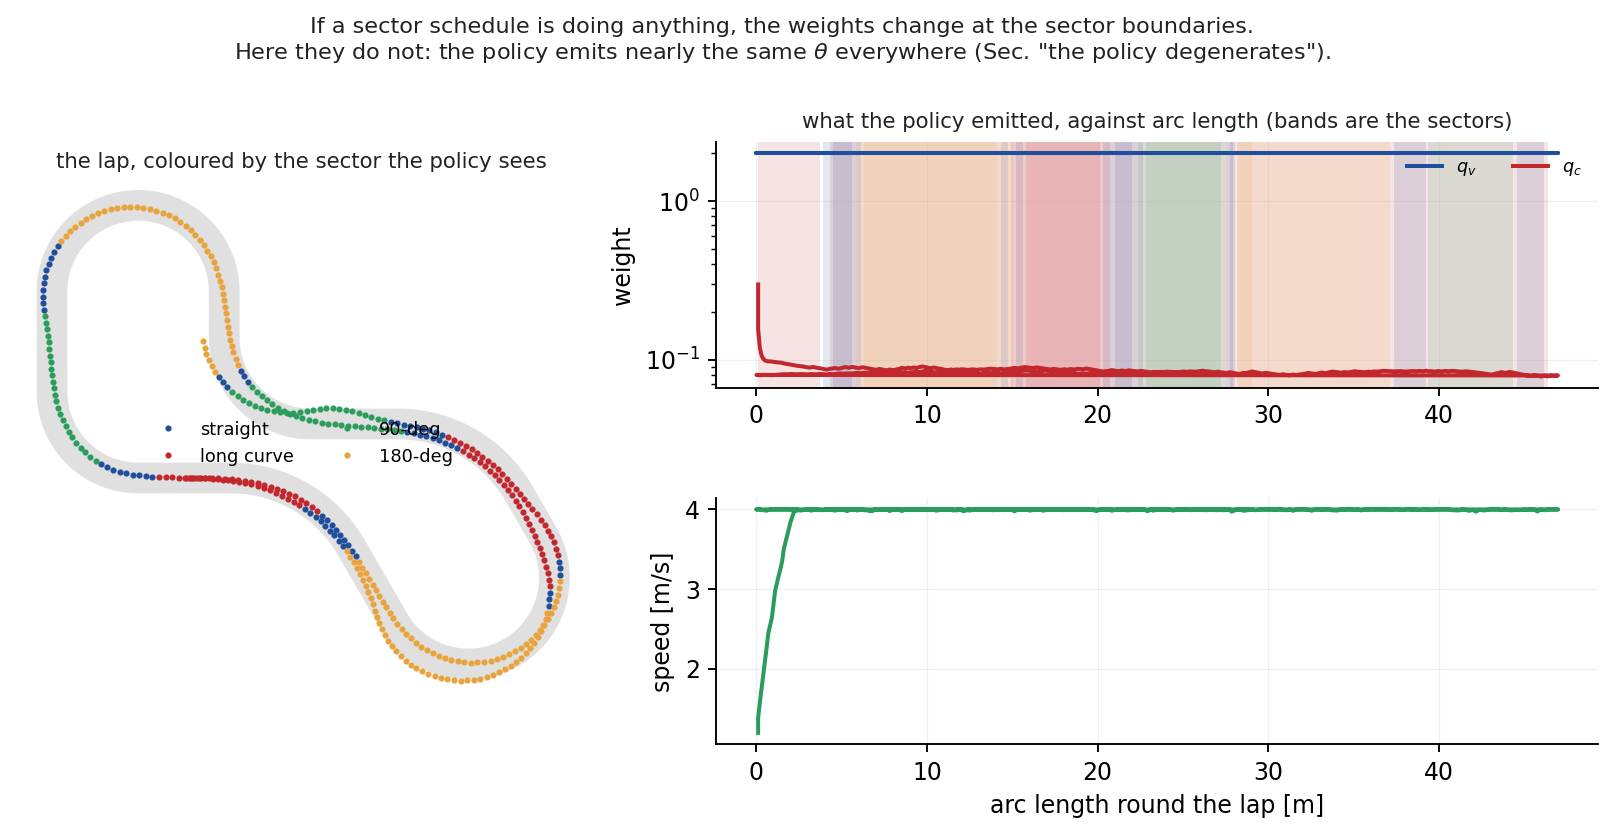
\includegraphics[width=\textwidth]{figures/driving_sectors.png}
  \caption{One lap of the four-sector circuit after ten episodes of online
  learning. \textbf{Left:} the driven path coloured by the sector the policy
  sees. \textbf{Right:} the weights it emitted against arc length, with the
  sectors as shaded bands, and the resulting speed. If a sector schedule were
  doing anything the weights would step at the band edges. They do not move at
  all --- $q_v$ is flat on its ceiling and $q_c$ flat near its floor for the
  whole lap --- which is Table~\ref{tab:sens} made visible.}
  \label{fig:driving}
\end{figure*}

Fig.~\ref{fig:driving} shows the same failure as a lap rather than a table: the
sector the policy sees changes eleven times round the circuit, and the weights
it emits do not step once.

\subsection{Two bugs a table could not show}
Drawing the emitted weights found, in sequence, two faults that twenty runs and
four summary rows had not.

\emph{A hard clip has no gradient.} We had bounded the policy output with
$\theta = \mathrm{clip}(\theta_0 + Gh)$. Wherever a weight sits on its bound,
$\partial\theta/\partial\phi = 0$, so the learner receives no gradient for that
component and can never bring it back: \textbf{the bound added for safety
switches off learning on the axis it bounds}. In the figure's first version
$q_v$ sat flat on the ceiling for an entire lap while only $q_c$ moved. The
bound is now a $\tanh$ squash into the same box, with the corresponding factor
chained into $\partial\theta/\partial\phi$.

\emph{Bounding an output is not a stopping criterion.} With the gradient
restored, the policy runs to the bound anyway --- the ratio reaches $22$ and the
episode return collapses. This is precisely the failure our companion work
documents for a \emph{single} global $\theta$~\cite{paper1}: the tuner optimises
a proxy past the point where the proxy is valid, with nothing to stop it. The
behaviour policy inherits it whole. A box constrains \emph{where} $\theta$ may
go, not \emph{whether it should keep going}, and the two are not the same
requirement.

That is the honest reading of Table~\ref{tab:gate}: the recurrent policy loses
to a hand-written schedule not because recurrence cannot represent the
behaviour, but because nothing in the loop tells it when to stop moving. A
trust region on $\theta$ is therefore a \emph{prerequisite} for this line of
work rather than an independent improvement to it, and we would not run another
policy comparison without one.

\section{Do named sectors pay for themselves?}
No. Table~\ref{tab:circuit}: four labels cost twice the parameters of three and
return a difference of \SI{7}{\centi\meter} at $0.8$ standard errors. We report
this because the sector taxonomy of Section~\ref{sec:sectors} is a genuine
correction to how curvature binning is described --- a \SI{90}{\degree} and a
\SI{180}{\degree} corner really are indistinguishable to it --- and because that
correction turns out not to change any outcome we can measure. Both facts are
worth having; only the first is usually reported.

\section{Limitations}
The policy comparison of Section~\ref{sec:gate} was run before the trust region
that Section~\ref{sec:adapt} argues it needs, so it measures a policy with no
stopping criterion against a schedule that cannot drift --- and should be read
as a statement about that pairing rather than about recurrence. The behaviour
result is on one opponent geometry, and the postures could not be separated by
it. Every scheduling result is on two synthetic tracks, and
Section~\ref{sec:circuit} is precisely a demonstration that two is not many --- the conclusion reversed between them, and
we have no basis for predicting a third. The overtake grid is one opponent
geometry. The plant is a kinematic bicycle
with a grip limit the controller does not model; results against a fitted-tyre
plant are not yet obtainable because the tuner does not survive it from the
default initialisation, which is a reward-design problem and not a scheduling
one. Nothing has run on a vehicle.

\bibliographystyle{IEEEtran}
\bibliography{refs}
\end{document}
